In this Chapter we aim at answering the question of why Statistical Mechanics is suitable to study economic systems. The essence of the answer is that, among other things, the techniques of Physics allows one to find the minimum energy configuration (or at least very good approximations) and the expectation value of certain quantities of interest in rather complicated settings, which is precisely what Economics could mostly benefit of. 

To the reader familiar with Statistical Mechanics, we draw attention to the fact that we present here the canonical ensemble not as a derivation from Thermodynamics, but as a systematic inference of a system's observables using Information Theory. Instead of assuming a system connected to a heat bath at a fixed temperature and employing the first postulate of Statistical Physics, we follow the work of Jaynes \cite{Jaynes57} and show that the Gibbs distribution is the solution for an inference problem with limited information.

\section{Statistical Mechanics as an inference problem}

Suppose we have an interacting system composed of $N$ particles, each with its own state $x_i$, which can be its position, velocity, orientation, decision of whether to buy a Mac or a PC, political affiliation, etc. The whole system can be fully characterized by the configuration vector $x = (x_1, \ldots, x_N)$ and we assume all the information we have about this system is the expected value of function $H(x)$, often called in physics settings the energy function. There are many questions we can ask about the system, for example what is the probability of this system being at a configuration $x$, or what is the expected value of another quantity $G(x)$. These questions are inference problems, and through Information Theory we can find out what is the best way we can answer them.

As proposed by Shannon \cite{shannon1948}, when faced with a choice of several probability functions that describe some data or phenomena, one should always opt for that which makes the least assumptions, given the constraints of the problem. This amounts to finding the probability distribution $p(x)$ that maximizes the \textbf{Shannon entropy}

%TODO: show the shannon entropy in an Appendix maybe?
\begin{equation}
    S[p] = - \int dx P(x) \log P(x)
\end{equation}
subject to the constraints imposed by observation. In our case, the constraint is that the energy function $H(x)$ has an average value $\langle H(x) \rangle = \int dx \, P(x) H(x) = E$ and we also have to impose the constraint that $P(x)$ is a probability distribution and therefore must be normalized, i.e., $\int dx \, P(x) = 1$. This means that to find $P(x)$ for our system, we must find $P(x)$ that maximizes the Lagrangian

\begin{equation}
\mathcal{L}[P] =  - \int dx P(x) \log P(x) + \alpha \left(\int dx \, P(x) - 1\right) + \beta \left( \int dx \, P(x) H(x) - E \right),
\end{equation}
where $\alpha$ and $\beta$ are the Lagrange multipliers of this maximization problem. 

We assume that at the maximum $P^\ast$ a small perturbation $P(x) + \delta P(x)$ does not alter the Shannon entropy. If we assume that all $\delta P(x)$ are independent (i.e., $\delta P(x)$ and $\delta P(x')$ are not correlated for every $x, x'$ in the support of the distribution), then for every $x$ this becomes a regular maximization problem. For every $x$, we must solve that $\frac{\delta \mathcal{L}(P)}{\delta P} (x)$ is equal to zero, that is:

\begin{equation}
\frac{\partial}{\partial P(x)}\left\{ -P(x) \log P(x) + \alpha \left(P(x) - 1\right) - \beta \left(P(x) H(x) - E\right) \right\} = 0, \quad \forall x  
\end{equation}

Solving this equation we have that for every value of $x$

\begin{align}
    & -\log P(x) - 1 + \alpha + \beta H(x) = 0 \Rightarrow \\
    & \Rightarrow  P(x) = e^{-1 + \alpha - \beta H(x)}
\end{align}

The Lagrange multipliers must be set so that the constraints are satisfied. For $\alpha$ we have that $e^{\alpha - 1}$ must normalize the probability distribution, i.e.

\begin{align}
   &  \int dx e^{-1 + \alpha - \beta H(x)} = 1 \Rightarrow \\
    & e^{1 - \alpha} = \int dx e^{- \beta H(x)} = Z
\end{align}

This normalization term is the sum over all the configurations and is called the \textbf{partition function}. For $\beta$ we must have that 

\begin{equation}
    \int dx H(x) \frac{e^{-\beta H(x)}}{Z} = - \frac{\partial}{\partial \beta} \log Z = E
\end{equation}

This means $\beta$ must be such that the average energy of the system is equal to the observed average $E$. However, suppose we have not actually observed $E$, all we know is that it is fixed to some  value. Then, because $E$ is given by the above equation for which the only degree of freedom is a Lagrange multiplier, all the possible values it can take are given by varying $\beta$ from 0 to $\infty$. We have finally arrived at the maximum entropy distribution for our inference problem, which is the \textbf{Gibbs distribution}

\begin{equation}
\label{eq:sm_gibbs}
    P (x | \beta) = \frac{1}{Z(\beta)} e^{-\beta H(x)}
\end{equation}

The extreme cases for $\beta$ give us an intuition on how the Gibbs distribution behaves. For $\beta = 0$, $P(x) = \frac{1}{Z}$, for all values of $x$: in this limit all configurations are equally likely, regardless of their energy $H(x)$. In the opposite case, when $\beta \to \infty$, $Z$ becomes more and more concentrated around its maximum point, where $E(x)$ is minimum, and eventually $P(x)$ collapses to a delta function around the minimum energy configuration, also known as the \textbf{ground state} (it can also have an equal mass in several points in the case of multiple minima). Therefore, in the full $\beta$ spectrum, the Gibbs distribution starts completely uniform in the space of all configurations and slowly coalesces around the minimum energy values. If we assume $H(x)$ is bounded, then for every finite value of $\beta$, the system has a finite probability of being in any configuration (what is known as ergodicity). Given a system described by the Gibbs distribution, the average value of another desired observable $G(x)$ is given by

\begin{equation}
g = \langle G(x) \rangle = \int dx G(X) \frac{1}{Z} e^{-\beta H(x)}
\end{equation}

Though we have called $H(x)$ the energy function for customary reasons, this function is in principle any arbitrary function of the system configuration that has a well defined average value. For most systems of interest we can always decompose it as a sum of small scale interactions, that is, we can write

\begin{equation}
    H(x) = \sum_{a} H_a (x_a),
\end{equation}
where $a$ represent minimal cliques, usually pairwise, where we can reduce the interactions in the system to microscopic interactions. In this way, the behavior of macroscopic quantities such as the average energy or any other observable we are interested depends on the sum of a large amount of simple interactions. 

Besides allowing for more realistic modelling, interactions have a side effect which is very well known to physicists but that don't appear frequently in economic debates: the existence of \textbf{phase transitions}. Instead of asking questions about the specific details of one equilibrium configuration, in Physics one usually explore the parameter space looking for sharp transitions in the behavior of average quantities such as average utility per agent, average number of goods traded, etc. Phase transitions are of special interest because they represent some of the most interesting phenomena a system can present, and indeed, many popular questions in Economics, such as business cycles, crisis, altruistic cooperation, etc, can be framed in terms of phase transitions.

We note that despite this being the standard theory for the canonical ensemble in Statistical Physics, we have not made so far any Thermodynamical (or any other "physical") assumptions. We have been describing generic systems where we simply applied the tools of Information Theory for the inference of a random variable for which we have limited information. There's nothing that limits us to using the Gibbs distribution only for gases in which the molecules interact according to the laws of Physics. This is the fundamental reason why Statistical Mechanics is so successful at explaining such a varied wealth of phenomena: despite being first developed via physical laws, its results are general.

The only real difference when dealing with a thermodynamical system is that when we plug the Gibbs equation back into the Shannon entropy we have

\begin{equation}
    S[P_G] = \log Z + \beta E,
\end{equation}
which is still general, but we can now use one of the Maxwell's relations to give $\beta$ a physical interpretation:

\begin{equation}
   \frac{1}{T} = \frac{\partial S}{\partial E} = \beta
\end{equation}

Therefore in physical systems $\beta$ is identified as the inverse temperature and when $T \to \infty$, the system is equally likely to assume any possible configuration. Likewise, when $T = 0$, the system is frozen at one of the ground states. 


\subsection{A simple example}

We make explicit the general nature of the Gibbs distribution deduced in this section by a simple example\footnote{This example was taken from the course notes of Nestor Caticha.} of a random variable $x$ that can take three values: -1, 0 or 1. We know it's average is $\langle x \rangle = m$. What is the best inference we can make for it's probability distribution $P(x)$? The Gibbs distribution is

\begin{equation}
   P(x) = \frac{e^{-\lambda x}}{Z(\lambda)},
\end{equation}
where $Z(\lambda)$ is given by:

\begin{equation}
   Z(\lambda) = \sum_{x\in \{-1, 0, 1\}} e^{-\lambda x} =
   1 + 2\cosh \lambda
\end{equation}

And $\lambda$ is given by

\begin{equation}
   m = - \frac{\partial}{\partial \lambda} \log Z(\lambda) =  - \frac{2 \sinh \lambda}{1 + 2 \cosh \lambda}
\end{equation}

Writing $u = e^{-\lambda}$ and writing the hyperbolic functions as $2 \cosh \lambda = e^\lambda + e^{-\lambda}$ and $2 \sinh \lambda = e^\lambda - e^{-\lambda}$ we have

\begin{equation}
   \frac{u - u^{-1}}{1 + u + u^{-1}} = m \Rightarrow 
   m + (m+1)u + (m -1) u^{-1} = 0
\end{equation}

Multiplying both sides of the equation by $u$, we have the second order equation $(m - 1) u^2 + m u + (m + 1) = 0$, for which the (positive) solution is

\begin{equation}
   u = \frac{-m - \sqrt{m^2 - 4(m^2 - 1)}}{2 (m - 1)}
\end{equation}

\begin{figure}[!ht]
  \centering
  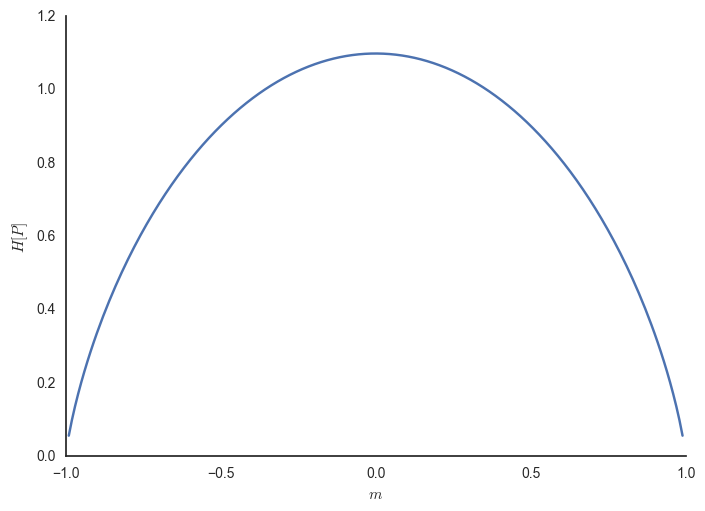
\includegraphics[width=0.4\textwidth]{figs_statmech/fig1a.png}
  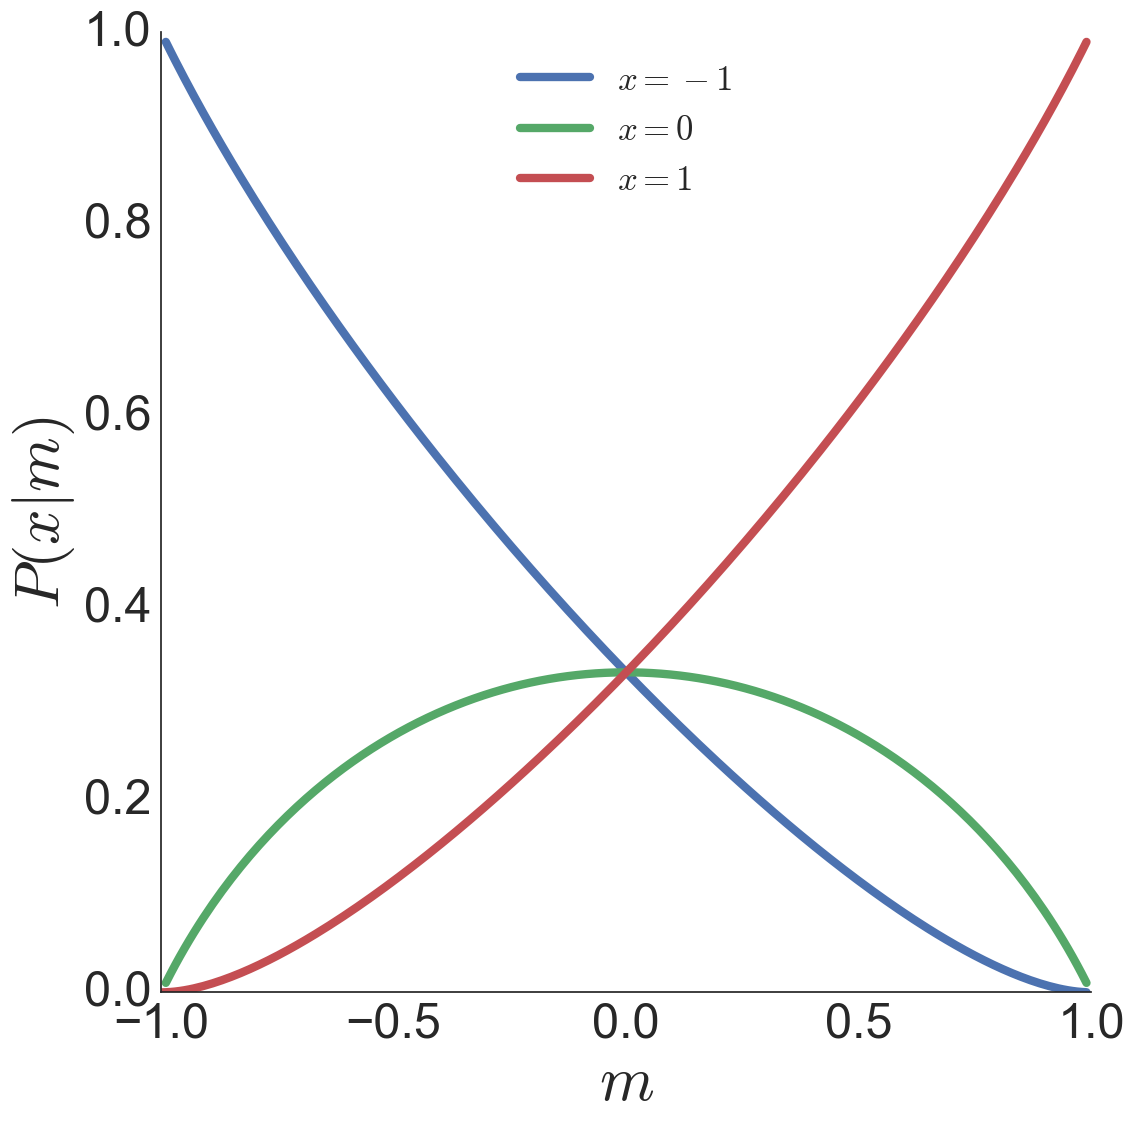
\includegraphics[width=0.4\textwidth]{figs_statmech/fig1b.png}
  \caption{\textbf{(Left)} Entropy $H[P]$ for the Gibbs distribution of a random variable $x$ that takes three values, -1, 0 and 1 as a function of its known average $\langle x \rangle = m$. \textbf{(Right)} Probability distribution $P_G(x|m)$ as a function of $m$ for each of the three values.}
  \label{fig:simple_example}
\end{figure}

And finally we find that $\lambda = -\log u$. We plot on Figure \ref{fig:simple_example} the entropy for the Gibbs distribution as a function of $m$ and the probability $P(x|m)$ for the three values. We see that as expected entropy is maximal when the three states are equally likely, and when $m = \pm 1$ the variable is fully identified, so the entropy goes to zero.


\subsection{Optimization Problems}

The Gibbs distribution offers a natural way of solving maximization problems: given a system that we know has energy function $H(x)$, its ground state is simply the distribution of states $x$ at zero temperature, or at $\beta \to \infty$. Likewise, we can find any quantity of interest $G(x)$ at the maximum by computing $\langle G(x) \rangle$ in that limit. 

This is certainly not the only way one can find solutions to optimization problems, however, framing it as a Statistical Physics problem has a couple of benefits, namely, if we accept approximate solutions, we can find them very close to the optimal in a time orders of magnitude smaller. Usually this is done using general purpose Monte Carlo algorithms to sample from the Gibbs distribution at a certain $\beta$ value and slowly increasing $\beta$ up (i.e., decreasing the system's temperature) until convergence, a technique known as \textbf{simulated annealing}. For well behaved convex functions there are certainly more efficient optimization algorithms, but Monte Carlo techniques are very robust and allow us to add constraints and interactions in the energy function without having to adopt an alternative maximization procedure.

As an example from \cite{mezard2004}, consider a conference planner that would like to distribute $N$ scientists in two available hotels. Scientists either like or dislike each other. We represent this by a positive interaction constant $J_{ij} = 1$ if $i$ and $j$ like each other and $J_{ij} = -1$ if $i$ and $j$ don't like each other. Scientists would then prefer to stay in hotels with their friends and not be in the same hotel with scientists they don't like. If we represent the hotel that a scientist is by $s_i = \pm 1$, the planner has to optimize for each scientist $i$ his utility

\begin{equation}
   u_i (\vec{s}) = \sum_{j=1, j\neq i}^N J_{ij} s_i s_j
\end{equation}

And then his problem is to find the configuration $\vec{s}$ which maximizes the total utility for all scientists, i.e.

\begin{equation}
   U(\vec{s}) = \sum_{i} u_i(\vec{s}) = \sum_{i, j} J_{ij} s_i s_j.
\end{equation}

For as little as 3 scientists, the problem can be frustrated: if all $J_{ij} = -1$ or if two are positive and one is negative, there are multiple ground states. For the general case, a brute force solution would require a search over $2^N$ configurations, which is unfeasible even for conferences with $N=100$ participants. However, with a Monte Carlo simulation we can find close approximations much more quickly.

This scenario, of course, is the Sherrington-Kirkpatrick model of a simple \textbf{spin glass}. Indeed, the theory of spin glasses are a very successful case in which complex systems with non regular patterns of interaction (also called \textbf{disordered systems}) can be studied, often solved analytically and exhibit very rich and interesting behavior.

These scenarios are not limited to physical systems: in portfolio optimization theory, one usually assumes that given a pool of possible financial assets, each with expected return $R_i$ and a covariance matrix $C$ for all assets, then given a fixed total assumed risk there is only one portfolio composition that maximizes the return and that a rational agent should adopt \cite{elton2009}. However, if one adds in the portfolio composition problem the requirement that any buy or sell operation carries a fee proportional to the value of the asset, then the optimization problem becomes glassy, presenting an exponential number of solutions to the number of available assets \cite{galluccio1998, gabor1999}. These aren't suboptimal solutions due to high temperature, but optimal portfolios a perfectly rational agent would choose.


\section{In Economics}

The utility of employing Statistical Mechanics to better model economic problems has not gone unnoticed by economists, even though it's usage is far from mainstream. It is most frequently used in interaction based models, in areas such as Game Theory, which arose precisely to deal with situations in which the decision of one agent affects the payoff of another, and rising microeconomic fields such as Social Interactions \cite{ScheinkmanSocialInt}. 

Probably the most influential work to show how a large interacting population can lead to unexpected outcomes is Schelling work on segregation \cite{schelling1971}, where two types of agents live in a city and all agents prefer to live in neighborhoods where their type is slightly more common than the other. This search for optimality will lead to complete segregation of agents, despite everyone preferring to live in mixed areas. In Schelling's words: "there is no simple correspondence of individual incentive to collective results". For a Statistical Mechanics treatment of Schelling's segregation model, we refer the reader to \cite{dall2008}.

One of the first major proposals of connecting Statistical Mechanics with Economics came from Santa Fe Institute's seminal work \textit{The economy as an evolving complex system} \cite{Anderson88, Arthur97}, which influenced physicists and economists alike. 

Later, in \cite{brock2001a} and \cite{brock2001b}, Brock and Durlauf describe an interacting model where each agent $i$ chooses between two binary actions $\omega_i = -1$ or $\omega_i = 1$ and his utility function has three terms: a private, deterministic term $u(\omega_i)$, one that interacts with other agents via a $J\omega_i \omega_j$ utility interaction and a random shock $\epsilon(\omega_i)$ whose distribution is given by the probability that $\epsilon(\omega_i = 1)$ is larger than $\epsilon(\omega_i = -1)$, given by a logistic distribution

\begin{equation}
P(\epsilon(1) - \epsilon(-1) > x) = \frac{1}{1 + e^{-\beta x}}
\end{equation}

In this setup the probability of agent $i$ choosing $\omega_i$ is given by

\begin{equation}
\label{eq:gibbs_brock}
P(\omega_i) = \frac{1}{Z} e^{\beta u(\omega_i)  + J \omega_i \left \langle\frac{1}{N}\sum_{j\neq i} \omega_j \right \rangle}
\end{equation}
where $Z$ is the normalization term. Writing $h = (u(1) - u(-1)) / 2$, then in equilibrium the expected value for the individual choice $m_i = m = \langle \omega_i \rangle$ is given by the implicit solution.

\begin{equation}
\label{eq:ferromagnet}
m = \tanh (\beta h + \beta J m)
\end{equation}

This is, of course, the solution for the mean field Ising model, which is exactly what the distribution probability \eqref{eq:gibbs_brock} represents. It is known that below a certain critical temperature $T_c$ there are three solutions: $m=0$ or $m = \pm m_0$, where $m_0$ can be found numerically. Above $T_c$, the only solution for equation \eqref{eq:ferromagnet} is $m=0$.

What is of note for this model is: \emph{(i)} how immediately useful framing an Economics problem into Statistical Mechanics can be. Economic problems can be modeled directly as well known systems, such as the Curie-Weiss model above. In this case, we now know that this economic interaction has three possible outcomes: when shocks to the consumer's utility are small, there are two possible rational behaviours: everyone chooses on average $m_0$ or $-m_0$. Otherwise, with large shocks, choice is essentially random. \emph{(ii)} How the current "classical equilibrium" mindset requires contrived choices for parameters. The Gibbs distribution was arrived at by assuming an specific family of shocks. By treating it as an inference problem, we arrived at the Gibbs distribution and the rich phenomenology that comes with by first principles.

Aside from problems that deal directly with the effects of interaction, Statistical Mechanics has also been used in Macroeconomics. In particular, Masanao Aoki studied many of its subject matters such as policy effectiveness, price stickness, business cycles and labor market by using stochastic processess \cite{AokiBook1, AokiBook2, AokiBook3}. He also repeatedly called attention to the fact that many economic settings are non self averaging, and the usual representative agent approach to Macroeconomics fails to grasp the full picture \cite{AokiSelfAvg}. 

\subsection{Statistical Equilibrium of Markets}

Besides the work of Masanao Aoki, Duncan Foley has also proposed a simple framework inspired by Statistical Mechanics for approaching market equilibrium which he calls \textbf{Statistical Equilibrium of Markets} \cite{Foley94, Foley96}, in which agents do not wait for a central authority to give them a price reference and instead make exchanges in a decentralized way. The only information an agent knows is whether he is willing to carry out a certain trade or not. With this simple rule, we are able to construct a model market with very interesting phenomenology.

Specifically, the model is composed of $M$ goods and $N$ agents which can be of $K$ different types ($K < N$). A transaction in this model is a vector $x = (x_1, \ldots, x_M)$, where an entry $x_\mu \in \R$ represents a good to be acquired in the trade, if $x_\mu > 0$ or traded away, if $x_\mu < 0$. Each type $k$ of agent has an offer set $A^k$ of transactions he is willing to make, which can be thought of single transactions or the results of a set of several trades. The nature of these sets is that they compose all transactions an agent would accept, regardless of feasibility. Therefore, one would expect that transactions of the type $x_\mu \geq 0$ for all goods $\mu = 1, \ldots, N$ are in the offer set for all groups $k$, because obviously no agent would shy away from free goods. 

The offer set is the core ingredient of this model, because it contains all the information about what the consumer is willing to trade for, without assuming much in terms of rationality: instead of knowing the optimal product bundle given all information available in the market, the consumer merely has to know if he likes a trade or not, a much better assumption. We can also write the offer set generated by an utility function in a straightforward manner: given an initial endowment $\omega$, the offer set $A_u$ for an utility function $u(y)$ is the set of all trades $x$ such that $u(\omega + x) > u(\omega)$. Companies and technologies are also included as agents, and the offer set of a company includes all the inputs it needs to operate its technology and all the resulting outputs. We assume that money is also a good, and therefore a company sets its prices defining how much money it is willing to get from the goods it offers. %%PRICE?

A market transaction is a matrix $X$ composed of transaction vectors for all agents, $X = (x_1, \ldots, x_N)$. Given a large enough market, we can also represent this matrix as frequencies: $h_k(x | X)$ is the frequency that transaction $x$ is carried by agents of type $k$ in $X$, where it must hold that $\sum_{x\in A_k} h_k (x | X) = 1$. If $N_k$ is the number of agents of type $k$ and $w_k = N_k / N$ is the proportion of type $k$ in the population, then we define the average excess demand vector for a transaction $X$ as

\begin{equation}
\label{eq:avg_excess_demand_foley}
    \bar{x} = \frac{1}{N} \sum_{i=1}^N x_i = \sum_{k=1}^K w_k \sum_{A_k} x h_k(x | X)
\end{equation}

The main question of this model is: what type of transactions are most likely to be carried out in this market? We assume we know nothing more about the market except the offer sets, and we require for consistency that the average excess demand is zero, that is, we would like that on average our market clears and that all transactions have a counterpart. Framing it this way, we end up with the problem that we want to find the distributions $h_k(x)$ best suited for our model given that they sum (or integrate) up to one and satisfy condition \eqref{eq:avg_excess_demand_foley}. This is an inference problem for which the solution is

\begin{equation}
h_k (x) = \frac{1}{Z_k} e^{-\pi \cdot x},
\end{equation}
where $Z_k = \sum_{x\in A_k} e^{-\pi\cdot x}$ is the partition function for group $k$ and $\pi$ are the Lagrange multipliers for the average demand restriction, which Foley dubbed the entropic prices. Because the vector $\pi$ guarantees the market clearing condition, they are considered the equilibrium prices that emerged from the market.

A practical application of the above setup is applying it to the labor market \cite{Foley96}. We can consider labor and money as the only two goods in the economy, which consists of two types of agents: workers, which have in their offer set either being unemployed or provide one unit of labor given that they receive at least more than a reservation wage, and firms, which demand one unit of labor and are willing to pay up to a certain amount. One of the consequences of this framing is that unemployment arises as a consequence of statistical fluctuation, showing it is present even in "efficient" markets. Furthermore, Foley shows that in this (decidedly stylized) scenario an employer subsidy to wages (i.e., giving them money to hire people) is more effective at reducing unemployment and increasing average salaries than a lump sum transfer to workers (complementing their wages with an extra).

One of the most interesting aspects of this Statistical Mechanics view on markets appears when one tries to understand what would a Walrasian equilibrium look like in this market. A configuration where all agents trade at the same prices, where agents with similar utility functions end up with the exact same consumption bundles, etc, would have zero entropy, which would require an enormous amount of information to arrive at from an initial configuration. This information reduction process is personified in the auctioneer figure, which, according to Foley, is as an impossible figure as the Maxwell demon, costlessly ordering an otherwise highly disordered system.


\section{The Role of Dynamics}

We end this chapter by touching briefly on the dynamical side of Statistical Physics. We have thus far described the role of inference in equilibrium configurations, where a global function for all the agents is maximized. However, there are other types of systems studied by Statistical Physics, such as stochastic dynamics, where we do not assume the system is at equilibrium, but explicitly write the probabilistic evolution rules for every particle. For example, the conference scenario described above could be replaced by one where we merely assume each scientist has a probability of changing hotels proportional to the difference in utility from being in one hotel or the other.

These methods can be equivalent to the approach described thus far if the dynamical rules converge to an equilibrium configuration, in which case they offer a different perspective for modelling economic situations, as is the case of the system we will study in Chapter \ref{cha:inequality}. Even if they surely converge to equilibrium though, glassy systems may take a very long time to do so, staying stuck in configurations which are seemingly stable but have higher energy than the ground state, a phenomenon known as \textbf{metastability}. This happens when the energy landscape of the system is very rugged and displays many local minima. This rugged landscape is frequently present when dealing with asymmetric interactions, as is the case of actual glasses and of some General Equilibrium dynamics, as we have mentioned in the last chapter. In these situations even if we have a theoretical proof of convergence, it may be useless for practical purposes because it is never reached.

However, it may be the case that the system never reaches an equilibrium. Furthermore, the behaviour of a particle may not even depend on a local energy function, as is the case in the Minority Game \cite{MinorityGames}: $N$ agents have to decide whether or not to go to a bar (or purchase a stock). Agents would like to go instead of staying home, however the bar is enjoyable only if it's not too crowded: if more than $L > N/2$ agents choose to go, agents prefer to stay home instead. However, if all agents decide simultaneously, they cannot check to see if the bar is full or not before going, and must make a decision only based on the knowledge of past attendances. It is called the Minority Game because it's advantageous to stay in the minority as the majority will always have made the worse choice. 

There are no deterministic strategies which solve the Minority Game, because if one existed all agents would adopt it and therefore it would stop being optimal. However, the agents can adopt mixed strategies to, on average, have a good payoff. This is well known from Game Theory, but the time aspect of the problem allow for agents with finite memory and a portfolio of strategies to be introduced \cite{MinorityGames99, MinorityGames00}.

Besides the minority game, some other examples are of note. Non-equilibrium dynamics are specially suitable for modelling Schumpeterian Economics, an area that mainly concerns with business cycles and "creative destruction" where innovation displace and  remove old business from market, both ideas proposed by Joseph Schumpeter. Examples of Statistical Physics applied to schumpeterian dynamics can be found in \cite{thurner}, where the authors show in a stylized economy that depending on the innovation rate, the economy will be either in a state of constant change akin to pure noise for high innovation rates, in a frozen configuration for low innovation rates or, more interestingly, in metastable states for intermediate innovation rates, staying still for long periods of time and then completely reshuffling.

In this thesis, we focus on systems at equilibrium, even in Chapter \ref{cha:inequality} where we begin by describing the dynamical rules for the economy and then study its steady state in terms of dynamical quantities. However, it's worth noting that this is not the only class of systems that can be studied with Statistical Physics, and out of equilibrium problems can also be useful in Economics. As time constrains our choices, following such interesting direction is left as an exercise for the reader.